\section[Theoretische Grundlagen]{Theoretische Grundlagen \normalsize{\cite{chempedia_nmr}}} 
\label{sec:physik}

Die Kernresonanzspektroskopie, auch Nuclear Magnetic Resonance Spectroscopy, kurz NMR genannt, ist eine spektroskopische Methode zur Strukturaufklärung von Molekülen. Sie wird in der Chemie, der Lebensmittelchemie, der Biologie und Biochemie, sowie in der Medizin genutzt. Mit Hilfe der NMR-Spektroskopie können neben der Strukturaufklärung auch quantitative Analysen, sowie die Untersuchung chemischer Gleichgewichte, chemischer Reaktionen und dynamischer Prozesse vorgenommen werden.
Grundlage dieser Spektroskopiemethode stellt die Wechselwirkung der magnetischer Kernmomente einer Probe mit einem äußeren Magnetfeld dar.

\subsection*{Voraussetzungen der Atomkerne}
Um mittels NMR-Spektroskopie Atomkerne untersuchen zu können, müssen diese eine Kernspinquantenzahl $I>0$ besitzen. Dies ist gegeben wenn mindestens eine der jeweilige Anzahlen an Protonen und Neutronen im Atomkern keine gerade Zahl ist. Entspricht die Anzahl der Neutronen und der Protonen jeweils einer gerade Zahl dann dann ist $I=0$. Eine Übersicht findet sich in Tabelle \ref{tab:messobjekte}.

% Table generated by Excel2LaTeX from sheet 'Daten'
\begin{table}[h!]
	\renewcommand*{\arraystretch}{1.2}
	\centering
	%\rowcolors{2}{white}{gray!25}
	\caption{Zusammensetzung von Atomkernen}
	\label{tab:messobjekte}
	\resizebox{\textwidth}{!}{
		\begin{tabulary}{1.2\textwidth}{C|C|C|C}
			\hline
			\textbf{Anzahl Protonen} & \textbf{Anzahl Neutronen} & \textbf{Kernspinquantenzahl} & \textbf{Detektierbar mit NMR ?}\\
			\hline
			gerade & gerade & $I=0$ & nein\\
			ungerade & ungerade & $I>0$ & ja\\
			ungerade & gerade & $I>0$ & ja\\
			gerade & ungerade & $I>0$ & ja\\
			\hline			
	\end{tabulary}
	}
\end{table}
\FloatBarrier
\vspace*{-5mm}
\subsection*{Kerndrehimpuls und magnetisches Moment}
Alle Atomkerne, außer gg-Kernen, besitzen außer einer Masse und einer Ladung einen von Null verschiedenen Eigendrehimpuls, den sogenannten Kernspin oder Gesamtdrehimpuls $\overrightarrow{P}$. Dieser Gesamtdrehimpuls bedeutet, dass ein Atomkern sich um seine eigene Achse dreht. Der Gesamtdrehimpuls $\overrightarrow{P}$ ist eine vektorielle Größe und verhält sich proportional zum magnetischen Dipolmoment $\overrightarrow{\mu}$. Der Proportionalitätsfaktor dieses Zusammenhanges wird gyromagnetisches Verhältnis genannt und mit $\gamma$ bezeichnet (siehe Gl. \ref{gl:gyro}). Die Werte für $\overrightarrow{\mu}$ entsprechen hierbei den Beträgen der magnetischen Momentvektoren. Dabei ist die Richtung dieser Momentvektoren in Abwesenheit eines äußeren Magnetfeldes beliebig und alle Kernzustände besitzen die gleiche Energie.

\begin{equation}
\label{gl:gyro}
	\overrightarrow{\mu} = \gamma*\overrightarrow{P}
\end{equation}

\subsection*{Kerne im statischen Magnetfeld}
Legt man nun ein äußeres, statisches Magnetfeld $\overrightarrow{B}_0$ an richtet sich der Gesamtdrehimpuls $\overrightarrow{P}$ der Kerne entlang der magnetischen Feldachse $P_z$ aus. Die Anzahl der möglichen Orientierungen hängt dabei von der Kernspinquantenzahl $I$ ab (siehe Gleichung \ref{gl:ksqz}). Der Gesamtdrehimpuls $\overrightarrow{P}$ ist gequantelt und nimmt daher ganz- oder halbzahlige Vielfache des \textsc{Plankschen} Wirkungsquantum $\hbar$ an. Aus Gleichung \ref{gl:gyro} folgt, dass demnach auch das magnetische Dipolmoment gequantelt ist und ebenfalls $2*I+1$ diskrete Einstellmöglichkeiten besitzt (siehe Gleichung \ref{gl:quantelung}).
Dieses gequantelte Verhalten der Atomkerne wird Richtungsquantelung genannt.
\begin{equation}
\label{gl:ksqz}	
	P_z = \left(2*I+1\right)*\hbar
\end{equation}

\begin{equation}
	\label{gl:quantelung}	
	\left| \overrightarrow{P} \right| = \frac{	\left| \overrightarrow{\mu} \right|}{\gamma} = \sqrt{I*\left(I+1\right)}*\hbar
\end{equation}

In Abbildung \ref{fig:energie} ist in einer Skizze dargestellt, in der gezeigt wird wie sich der Gesamtdrehimpuls $\overrightarrow{P}$ ohne und mit einem äußeren, statischen Magnetfeld verhält. Zu erkennen ist, dass es bei angelegten Magnetfeld zu parallelen und antiparallelen Ausrichtungen der Richtungsvektoren kommt und eine Aufspaltung in verschiedenen Energieniveaus erfolgt. Da die parallele Ausrichtung energetisch günstiger ist, sind entsprechend mehr Kerne parallel als antiparallel im äußeren Magnetfeld ausgerichtet.

\begin{figure}[h!]
	\centering
	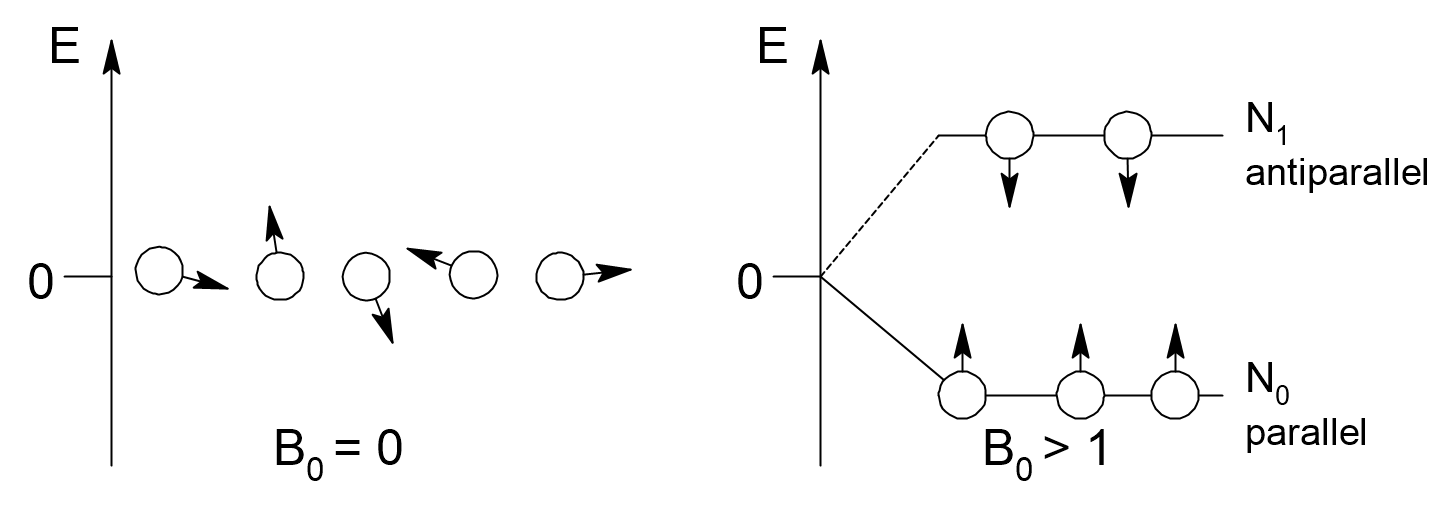
\includegraphics[width=0.8\textwidth]{img/energiediagramme}
	\caption{Energie der Kerne im Magnetfeld und Besetzung der Energieniveaus}
	\label{fig:energie}
\end{figure}
\FloatBarrier
%Ende

Da das äußere Magnetfeld $\overrightarrow{B}_0$ auf das magnetische Dipolmoment $\overrightarrow{\mu}$ ein Drehmoment ausübt beginnt dieses um die Richtung von $\overrightarrow{B}_0$ mit der sogenannten Lamorfrequenz $\omega_L$ zu präzedieren. Diese Lamorfrequenz ist an dieser Stelle mit der Resonanzfrequenz gleichzusetzen und funktioniert aufgrund der Drehimpulserhaltung. Die sich daraus ergebende Resonanzbedingung ist in Gleichung \ref{gl:resonanz} dargestellt.

\begin{equation}
	\label{gl:resonanz}
	\omega_i = \omega_L = \gamma * B_0
\end{equation}

\subsection*{Kernresonanz und Relaxation}
Bei elektromagnetischer Einstrahlung entsprechend der Resonanzbedingung \newline \mbox{(siehe Gl. \ref{gl:resonanz}) } kommt es sowohl zu Übergängen vom energieärmeren in das energiereichere Niveau (Absorption) als auch in umgekehrter Richtung (Emission). Dabei überwiegt der Vorgang der Absorption. Während dem Hauptprozess der Absorption wird Energie vom Kern aufgenommen und zum Übergang in einen höheren Energiezustand verwendet. Diese Energieabsorption kann zusammen mit ihrer Intensität als Signal gemessen werden und kann zusätzlich auf die Konzentration der Probe am gemessenen Isotop schließen lassen. Am Ende der Energiezufuhr durch einen Sendeimpuls einer Senderspule kommt es zur "`Sättigung"' und alle Kernspinniveaus  besitzen die gleiche Energie. Darauf folgt der Vorgang der Relaxation. Innerhalb dieses Vorganges wird die absorbierte Energie durch die Einstrahlung wieder freigegeben und mit Hilfe einer Empfängerspule gemessen. Innerhalb dieses Prozesses kann zwischen longitudinaler und transversaler Relaxation unterschieden werden. Aus den aufgenommenen Messsignalen wird durch einen Computer mittels \textsc{Fourier}-Transformation das auszuwertende NMR-Spektrum erzeugt.